\documentclass[border=8pt]{standalone}
\usepackage{fontspec}\usepackage{tikz}
\usetikzlibrary{arrows.meta,positioning,fit,backgrounds}
\definecolor{NouOrange}{HTML}{FA4D1F}\definecolor{NouBlack}{HTML}{000000}
\begin{document}
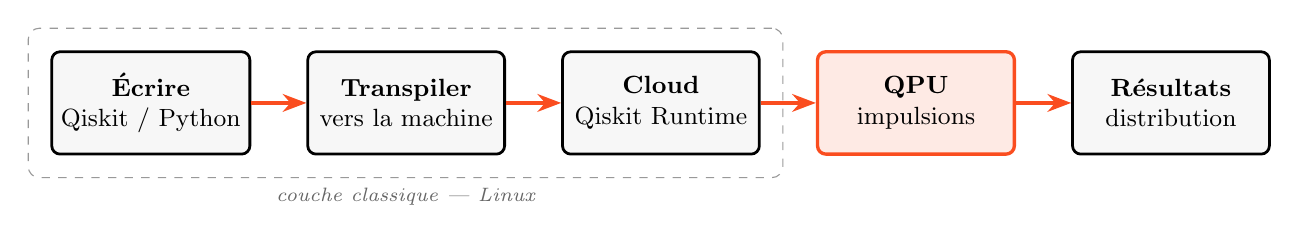
\begin{tikzpicture}[font=\sffamily,node distance=0.7cm,
  s/.style={draw=NouBlack,line width=1pt,rounded corners=3pt,align=center,minimum width=2.5cm,minimum height=1.3cm,fill=black!3,font=\small}]
  \node[s] (ecr) {\textbf{Écrire}\\Qiskit / Python};
  \node[s,right=of ecr] (tr) {\textbf{Transpiler}\\vers la machine};
  \node[s,right=of tr] (cl) {\textbf{Cloud}\\Qiskit Runtime};
  \node[s,right=of cl,fill=NouOrange!12,draw=NouOrange,line width=1.2pt] (qpu) {\textbf{QPU}\\impulsions};
  \node[s,right=of qpu] (res) {\textbf{Résultats}\\distribution};
  \foreach \a/\b in {ecr/tr,tr/cl,cl/qpu,qpu/res}{\draw[-{Stealth[length=3mm]},NouOrange,line width=1.3pt] (\a) -- (\b);}
  \begin{scope}[on background layer]
    \node[draw=NouBlack!40,dashed,rounded corners=4pt,fit=(ecr)(tr)(cl),inner sep=8pt,label={[font=\scriptsize\itshape,NouBlack!60]below:couche classique — Linux}] {};
  \end{scope}
\end{tikzpicture}
\end{document}
